\section{System Implementation}

The Graffiti API is general enough that during the course of our development
we experimented with many different implementations including
a traditional centralized implementation, a peer-to-peer implementation where user
data was stored across users' browser storage, and an implementation that
bootstrapped off existing storage providers like Dropbox and Solid
tied together with a BitTorrent-like tracker service.

While we touch on these other implementations briefly,
the description below is focused primarily on our \emph{canonical} implementation
that we believe, of the options we pursued, strikes
the best balancce between usability, efficiency, and data ownership.
This canonical implementation is also where we focused most of our development effort.
However it is certainly not the only way to implement Graffiti and
in fact one of its strengths is that it is not tied to any particular
implementation.
We imagine a future with coexisting implementations
of Graffiti with bridges between them, much like how the internet protocol
can be built on top of many different physical networks:
copper, optical fiber, radio wi-fi and satellite, etc.

Our canonical implementation of Graffiti consists of four system components:
identity providers, storage pods, a core client library, and a frontend framework.
The identity providers and storage pods are independent servers
--- many of them can exist, and a user can freely choose which ones to use, or even host their own.
A user interact seamlessly with users who use different identity providers and storage pods,
and can migrate their own identity or data between them at any time, preventing lock-in to these services.
The core client library is client-side code that makes
run in parallel while the other
layers build on top of them.

[ Insert system diagram here ]

\usepackage{cleveref}
\subsection{Identity Provider}
\label{identity-provider}

To achieve persistent user identities in Graffiti
we use the Solid OpenID Connect specification~\cite{solid-oidc}.
On the surface level, this provides Graffiti applications
with an single-sign-on interface akin to a "Sign In with Google" button
as shown in Figure~\ref{fig:solid-oidc}.
However, while most single-sign-on interfaces only authorize
the client application to interface with a single server,
Solid OIDC authorizes the client application
to communicate with any server on the user's behalf which
is necessary for users to pull data from the multiple storage pods
we describe in~\cref{storage-pods}.
Additionally, the user can choose from any compliant
Solid identity provider including one they host themselves.

\begin{figure}
\label{fig:solid-oidc}
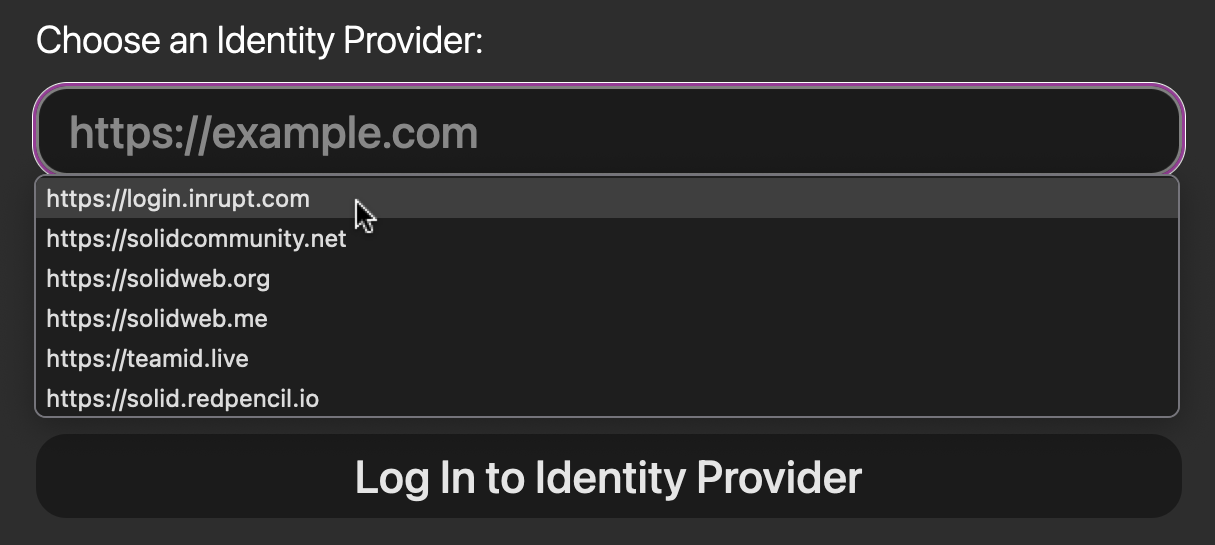
\includegraphics{paper/system/solid-oidc.png}
\caption{A user can choose from several common Solid identity providers
or manualy enter a custom one.}
\end{figure}

The Solid OIDC specification also provides
each user with a webId, a globally unique and human-readable URL
that can be shared like a username or an email address.
At this URL, the user can store a small amount of public data
which we use to implement "delegation".

There are multiple open source implimentations of Solid OIDC servers,
client libraries, and authorization libraries that we use out of the box.
While these implimentations were useful for getting started,
they have some limitations that we would eventually like to address.
None of thse limiations are necessarily at odds with the Solid OIDC
specification, they are either not implemented in the current libraries
or not fully laid out in the specification.

For one, the most popular browser client library is quite large
because it includes other Solid semantic web features not relevant to Graffiti.
This leads to large bundle sizes that can be slow and make Graffiti inaccessable
to users with limited data plans.

Additionally, existing OIDC servers generate their own
webIds, which are often verbose,
\emph{e.g.} \url{janedoe.solidcommunity.net/profile/card#me}.
There is no reason why a user could not come with their own, simple, domain name, for example
\url{id.janedoe.com}, similar to the AT Protocol~\cite{bluesky}. This would also give the users the ability
to switch identity providers while maintaining their identity.
It is not also currently easy to generate throwaway webIds
which could be useful for one-time or anonymous interactions.

Finally, once you are logged in with a webId users are
granted full access rights. Incorporating scoped access rights
into the Solid OIDC specification would allow users to comfortably
interact with new applications without the risk of exposing or losing
their data.

\subsection{Storage Pods}
\label{storage-pods}

Graffiti data is stored and served by storage \emph{pods}.
A person can choose which pod or pods they want to host their data
and at any time migrate to a different pod including one they host themselves.
Users can consume data from any pod.
Altogether, this prevents users from being locked into any one storage provider.

Pods provide two main functionalities:
\begin{enumerate}
\item CRUD style operations for creating, retrieving, updating and deleting data.
\item A \emph{discover} method for querying for data within a pod subject to soft access control (channels)
and hard access control (access control lists).
\end{enumerate}

Almost any online storage provider fulfills the first requirement,
and therefore we have demonstrated that it is possible to implement Graffiti on top both Dropbox and Solid.
However, to implement discovery on top of such services requires a seperate
bittorrent-like \emph{tracker} service and an extremely large number of network requests
to the storage providers that is both expensive and slow.

Therefore, we opted to build our own pods as the primary implementation of Graffiti.
However this suggests that many implementations can coexist and bridges
could be built between them.

\subsubsection{Data Model}

Like ActivityPub, social data is assumed to be comprised of atomic JSON objects.
In addition to their JSON value, they also contain the following metadata
\begin{itemize}
\item \emph{channels} a list of URIs that the object is associated with.
\item \emph{access control list} a list of webIds of users allowed to view the object, or undefined if the object is public.
\item \emph{last modified time} the time the object was last modified which is used for caching.
\item \emph{webId} the webId of the user who created the object.
\item \emph{name} a usually randomly-generated string used to identify the object.
\item \emph{storagePod} the URL of the pod that the object is stored on.
\end{itemize}

\subsubsection{CRUD}

An object is uniquely identified by its storagePod, owner, and name
therefore the URL of an object is of the form \texttt{storagePod/webId/name}.
Users can use PUT, GET, PATCH, and DELETE methods to create, retrieve, update, and delete objects
at these URLs.

PUT, PATCH, and DELETE operations return the object before modifactaion if it exists.

PUT, PATCH, and DELETE operations can only be performed by the owner of an object
- remember that any collaboration or moderation is done by annotating object with new objects.
To authenticate, a user must be logged in with their identity provider.
GET operations do not require authentication unless the object is access controlled.

PATCH operations are implemented with JSON Patch.




One interesting thing is that it shifts the cost of data storage to the poster
rather than the viewer.
For example, if a post goes viral and is viewed by millions of people,
the cost of serving the data is distributed among the millions of viewers
This is unlike traditional social media where the cost of serving the data
is born by the poster.


However for scalability reasons,
we built our own pods that are more specialized for Graffiti.

Graffiti pods offer traditional HTTP methods: PUT, GET, REST,
They also have a `discover' which allows users to find data across the pod.
Finally there are methods

\subsubsection{REST Methods}

Users

At URLS of the form `storagePod/webId/name'.
For example, if the pod is \url{https://pod.graffiti.garden},
the user's webId is \url{https://alice.example.com},
and the object is named \texttt{12345},
the URL would be \url{https://pod.graffiti.garden/https\%3A\%2F\%2Falice.example.com/12345}.

Objects have a value, channels, access control list, and last modified time.
The value is returned in the body,
and the others are returned in headers.
The name and webId are aparent from the URL.

PUT, GET, DELETE, and PATCH are supported.

When putting an object the JSON is in the body.

When getting an object, the object is returned in the body.



When getting an object, channels and access control lists are returned only
if the user is the creator and not for other users.

Patches are done with JSON patch. Seperate patches are passed for value, channels, and acl.

When putting, deleting, or patching and a previous object exists, it is
returned in the response.

\subsubsection{Discover}

\subsubsection{Zero-Knowledge Discovery}

held in storage pods which store and serve data and have minor roles in
limiting access control and filtering content according to queries.

\subsection{Core Client Library}

In addition to interfacing with identity providers,
and storage pods, the core library provides additional functionality
around delegation, announcements, filtering and caching.

The library is written in Typescript and can be used in both the browser and node.js.

\subsubsection{Delegation}

Many decentralized systems use public key cryptography to sign messages,
however this can mean that anything a user writes is undeniable and can
possibly be leaked even if it was meant to be private as we discussed in X.
Instead we use delegation, whereby a user chooses.

Therefore, the client application needs to know which pods a user has delegated
to so that they can know whether to trust the data.

As we saw in \cref{identity-provider}, the Solid OIDC specification
allows a user to store some amount of data at their webId.
That data is a URL which points to a Graffiti object owned by the user
on some pod, and includes global settings.
These settings include a list of

The settings also include forwarding rules which allow a user to

The verification of these settings is done by the client core library.

\subsubsection{Announcements}

When an application makes a \texttt{discover} request to a pod, that request
only returns results from that specific pod. However, users may have posted across
multiple pods. Therefore when a user makes a post in one pod, the client library
also puts "announcements" in several well known pods of the users choosing.
This way, when a user makes a \texttt{discover} request, their client first
makes \texttt{discover} requests for announcements in the users known pods
and then makes \texttt{discover} requests from the pods that have been found.
So long as there is some overlap in the well known pods that users have chosen,
the user will be able to see all of their posts.

These announcements are graffiti objects like any other and so more metadata
or announcement-like objects can be added over time to improve efficiency or
discoverability. For example, it may not be necessary.

\subsubsection{Filtering}

Types help to provide a better software experience.
Anyone can host a pod and so the results are not necessarily trustworthy.
So

\subsubsection{Caching}

A users profile can be

\subsection{Front End Tooling}

\subsection{Alternative Implementations}

\subsubsection{Bootstrapping off of Existing Storage Providers}

It is possible to implement Graffiti on top of existing storage providers,
like Dropbox or Solid. When a user posts an object, that object is stored in
a large folder of all the user's objects. Then that object is symlinked into
folders for each channel the user wants to post the object to.

Unlike in our canonical implementation, it is not possible to query for
all objects in a channel by a particular storage provider. Instead, a
separate BitTorrent-like \emph{tracker} service is required to
point users to the appropriate storage provider channel.

Using a commercial storage provider like Dropbox allows for access control but only if users
have a Dropbox account, which locks users into a proprietary service.
Solid does not have this problem. In fact, it is not possible to use the Dropbox API
without being used into a Dropbox account, but it is possible to use the Solid API
without being locked into a Solid account.

The primary reason for not pursuing this implementation is that it requires
an extremely large number of network requests to the storage providers
that is both expensive and slow. Additionally, these storage providers
do not support querying for objects in a particular channel and instead
all the filtering has to be done client-side.

While we expect some users of our canonical implementation to host their own pods,
many will use large pods hosted by others, much like Email or Mastodon.
Only a single network request is required per pod to retrieve all objects in a channel,
whereas a seperate request is required per user and event per object in the Dropbox model.

\subsubsection{Peer-to-Peer Implementation}

While this may have been possible in the PC era, it is not possible in the mobile era.
Most users are not online all the time and can lose their devices or accidentally wipe their data.

